%
%   Hotpy Documentation
%

\documentclass{book}

\usepackage{amsmath}
\usepackage{graphicx}
\usepackage{hyperref}
\usepackage{esint}

\hypersetup{colorlinks, allcolors=blue, linkcolor=magenta}

\def\version{1.2}
\def\package{pyro-\version{}}
\def\lpackage{\package{}.tar.bz2}
\def\wpackage{\package{}.zip}
\def\classes{4}
\def\species{79}


\begin{document}

\frontmatter
% Begin Title Page
\begin{center}
\vspace{2in}

\includegraphics{fig/PYro_Black_MedSmall}\\
\vspace{0.5in}
{\Huge PYro}\\
\vspace{0.5in}
{\huge Thermodynamic Computational Tools for Python}\\
\vspace{0.2in}
Version \version{}\\
\vspace{1in}
{\Large Christopher Martin}\\
{\large Assistant Professor of Mechanical Engineering}\\
{\large The Pennsylvania State University, Altoona College}\\
\vspace{1in}
{\large April 2016}
\end{center}
% End Title Page
\pagebreak

\begin{center}
\mbox{}\\
\vspace{3in}
Thanks go to the talented Janet Montgomery\\
for developing the PYro icon.\\
\vspace{0.5in}
\url{https://www.behance.net/janetmontgomery}
\end{center}

\pagebreak

\tableofcontents
\mainmatter

\chapter{Introduction}\label{sec:intro}
\section{What is PYro?}
PYro is a flexible platform for conveniently working with gobs and gobs of thermodynamic data in scripts and at the command line in Python.  The intent behind PYro is probably best described with an apocryphal story.

\begin{verse}
There once was a student\\
with work ethic prudent\\
she scripted to speed her work.

In Python t'was coded,\\
so when it was loaded,\\
she could all the tedium shirk.

A thermodynamic\\
fluid mechanic\\
problem she had solved.

Her colleagues were avid\\
she share the package\\
frustration to resolve.

Good, was the mood.\\
Researchers all cooed,\\
until she read her mail.

With no contradiction,\\
viscosity-friction;\\
with it her package would sail.

She furiously typed\\
new modules to write.\\
The people, they must be heard.

What thanks had it gotten?\\
why, STEAM she'd forgotten!\\
Without it, the code was absurd.

Downtrodden indeed,\\
she sat at the screen,\\
multiphase soon to add.

Though coffee was drunk\\
and sleepless nights sunk,\\
her code, it really was bad!

The syntax was rambling\\
no hope of unscrambling\\
the endless nonsensical edits.

Compatible, reverse,\\
a programmer's curse\\
no fixing - it's time to shred it.

``I'm done,'' she then plead.\\
To the airport, she fled.\\
``I'll fly off to someplace that's random.''

Her useful creation\\
was once a sensation;\\
forgotten and now is abandoned.

Her colleagues still moan,\\
``Please pick up your phone!\\
Your software, it just isn't working.''

Ye coders beware\\
the fate most unfair,\\
within all your projects is lurking.
\end{verse}

With a flexible framework that allows users to define their own data and even their own classes, the hope is that over time PYro will graudally be extended to do the jobs that people need most, but in a way that is ``Pythonic'' and extensible.  In that way, PYro is distinguished from other excellent thermodynamic resources (like Cantera) by its emphasis on being application agnostic.  

PYro is easily installed using a standard setup script, convenient to use from the command line, but also highly configurable.  To get a feel for how easy PYro is to use, look at section \ref{sec:start}.

\underline{What can PYro do?}  The PYro classes supply methods for calculating most common thermodynamic properties from temperature and pressure such as density, enthalpy, entropy, internal energy, molecular weight, specific heats, specific heat ratio, and specific volume.

While version 1.1 included only ideal gas data, version 1.2 includes properties of water and steam.  There are plans to include refrigerants in later releases.

The addition of the psolve() function to all classes makes property inversion possible.  In other words, it is possible to determine the pressure and temperature at which a substance will have a given entropy and enthalpy.  This comes in handy for cycle analysis and flame temperature calculations.

\underline{What can't PYro do?}  In addition to many others, all of the species supported by the \href{http://combustion.berkeley.edu/gri-mech/}{GRIMech reaction database} are included, but the corresponding chemical kinetic data are not.  While this could possibly change one day, \href{http://cantera.github.io/docs/sphinx/html/index.html}{Cantera} already offers excellent chemical kinetics support, so adding this functionality is not a priority.  This is an example where Cantera is probably just a better tool for the job than PYro.

It is also worth noting here that psolve() is not as robust as it should be for steam in the vicinity of phase changes.  The abrupt discontinuity in properties causes problems for the Newton algorithim or which psolve is built.  This will definitely be addressed in the future.

\section{Getting Started}\label{sec:start}
Whether you are just getting started or you are curious whether PYro will work for your application, this section should be what you need.

First, we begin with a bit of preparation.
\begin{verbatim}
>>> import pyro
>>> import matplotlib.pyplot as plt
>>> import numpy as np
\end{verbatim}

It can be very simple to get some quick information.
\begin{verbatim}
>>> O2 = pyro.get('O2')
>>> O2.cp(T=432)
0.95049900128261733
\end{verbatim}

It can be very simple to get lots of quick information.
\begin{verbatim}
>>> T = np.arange(300,4000,10)
>>> plt.plot(T, O2.h(T))
>>> plt.xlabel('Temperature (K)');plt.ylabel('Enthalpy (kJ/kg)')
>>> plt.grid('on')
\end{verbatim}

\begin{figure}[h!]
\begin{center}
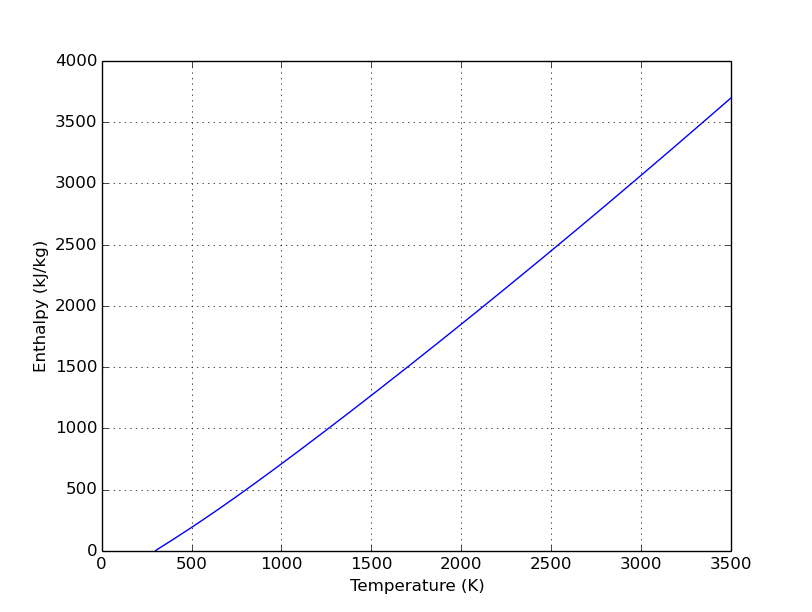
\includegraphics[width=.75\linewidth]{fig/o2h}
\caption{Enthalpy of diatomic oxygen.}
\end{center}
\end{figure}

Methods are available to calculate a number of common thermodynamic quantities; density (\verb|.d|), enthalpy (\verb|.h|), entropy (\verb|.s|), internal energy (\verb|.e|), molecular weight (\verb|.mw|), specific heats (\verb|.cp| and \verb|.cv|), specific heat ratio (\verb|.k|), and others.

Data are available for mixtures too.  In addition to the typical methods for calculating properties, the \verb|mixture| class provides methods to interrogate the mass, molar, and fractional mass and molar contents.
\begin{verbatim}
>>> air = pyro.get('air')
>>> air.M()
{u'N2': 21.88, u'Ar': 0.373, u'CO2': 0.013, u'O2': 6.704}
>>> air.N()
{u'N2': 0.7810547809262709, u'Ar': 0.009337138279763693, 
u'CO2': 0.00029539076790238467, u'O2': 0.20950785654462042}
>>> air.Y()
{u'N2': 0.7552640662754573, u'Ar': 0.012875388332758024, 
u'CO2': 0.0004487400759406282, u'O2': 0.23141180531584396}
>>> air.X()
{u'N2': 0.780902374928423, u'Ar': 0.009335316338574262, 
u'CO2': 0.0002953331287638292, u'O2': 0.20946697560423902}
>>> air.d( T=400, P=2.0 )
1.741805229300913
\end{verbatim}

The \verb|info()| function prints a summary of all available species.
\begin{verbatim}
>>> pyro.info()
  PYro
Thermodynamic computational tools for Python
version: 1.2
-------------------------------
ID      Modified    Type
-------------------------------
Ar      4/7/2016    igfit
Ar+     4/7/2016    igtab
Ar2     4/7/2016    igtab
C       4/7/2016    igfit
C2H     4/7/2016    igfit
C2H2    4/7/2016    igfit
C2H3    4/7/2016    igfit
C2H4    4/7/2016    igfit
C2H5    4/7/2016    igfit
C2H6    4/7/2016    igfit
C3H7    4/7/2016    igfit
C3H8    4/7/2016    igfit
CH      4/7/2016    igfit
CH2     4/7/2016    igfit
CH2(S)  4/7/2016    igfit
-------------------------------
ID      Modified    Type
-------------------------------
CH2CHO  4/7/2016    igfit
CH2CO   4/7/2016    igfit
CH2O    4/7/2016    igfit
CH2OH   4/7/2016    igfit
CH3     4/7/2016    igfit
CH3CHO  4/7/2016    igfit
CH3O    4/7/2016    igfit
CH3OH   4/7/2016    igfit
CH4     4/7/2016    igfit
CN      4/7/2016    igfit
CO      4/7/2016    igfit
CO2     4/7/2016    igfit
Cl      4/7/2016    igtab
F       4/7/2016    igtab
F2      4/7/2016    igtab
-------------------------------
ID      Modified    Type
-------------------------------
F5      11/6/2015   mixture
FK      4/7/2016    igtab
FN      4/7/2016    igtab
FO      4/7/2016    igtab
H       4/7/2016    igfit
H2      4/7/2016    igfit
H2CN    4/7/2016    igfit
H2O     4/7/2016    igfit
H2O2    4/7/2016    igfit
H35     11/6/2015   mixture
HCCO    4/7/2016    igfit
HCCOH   4/7/2016    igfit
HCN     4/7/2016    igfit
HCNN    4/7/2016    igfit
HCNO    4/7/2016    igfit
-------------------------------
ID      Modified    Type
-------------------------------
HCO     4/7/2016    igfit
HNCO    4/7/2016    igfit
HNO     4/7/2016    igfit
HO2     4/7/2016    igfit
HOCN    4/7/2016    igfit
He      4/7/2016    igtab
He+     4/7/2016    igtab
I       4/7/2016    igtab
I2      4/7/2016    igtab
IK      4/7/2016    igtab
Kr      4/7/2016    igtab
N       4/7/2016    igfit
N2      4/7/2016    igfit
N2O     4/7/2016    igfit
NCO     4/7/2016    igfit
-------------------------------
ID      Modified    Type
-------------------------------
NH      4/7/2016    igfit
NH2     4/7/2016    igfit
NH3     4/7/2016    igfit
NNH     4/7/2016    igfit
NO      4/7/2016    igfit
NO2     4/7/2016    igfit
Ne      4/7/2016    igtab
Ne+     4/7/2016    igtab
O       4/7/2016    igfit
O2      4/7/2016    igfit
OH      4/7/2016    igfit
Rn      4/7/2016    igtab
S       4/7/2016    igtab
S2      4/7/2016    igtab
S3      4/7/2016    igtab
-------------------------------
ID      Modified    Type
-------------------------------
S4      4/7/2016    igtab
Xe      4/7/2016    igtab
air     11/6/2015   mixture
steam   12/24/2015  if97
\end{verbatim}

When called with the name of a species, it returns more specific information information. 
\begin{verbatim}
>>> pyro.info('HCO')
***
Information summary for substance: "HCO"
***
Uses class:   igfit

Loaded from:  C:\Users\crm28\WinPython-64bit-2.7.10.2\python-2.7.10.amd64\lib\site-packages\pyro\data\HCO.hpd

Last updated: 10:07 December 5, 2015

These data are adapted from the GRI-Mech website,
http://www.me.berkeley.edu/gri-mech/
and are credited to
B.J. McBride, S. Gordon, and M.A. Reno, 'Coefficients for Calculating
Thermodynamic and Transport Properties of Individual Species', NASA Report
TM-4513, October 1993
A. Burcat and B. McBride, '1994 Ideal Gas Thermodynamic Data for
Combustion and Air- Pollution Use', Technion Report TAE 697, December 1993
Adaptation by Chris Martin (c)2015.
Units are supplied in: energy kJ temperature K mass kg molar kmol

>>>  pyro.info('air')
***
Information summary for substance: "air"
***
Uses class:   mixture

Loaded from:  C:\Users\crm28\WinPython-64bit-2.7.10.2\python-2.7.10.amd64\lib\site-packages\pyro\data\air.hpd

Last updated: 10:34 December 5, 2015

The composition of air is taken from section 14 page 20 of the the CRC
Handbook of Chemistry and Physics 96th ed, 2015-2016.
www.hbcpnetbase.com
Trace gases (those present in less than 0.01% by volume) are neglected, as
they will not contribute substantially to the thermodynamic properties.
Original work is credited to:
COESA, "U.S. Standard Atmosphere, 1976", U.S. Government Printer Office,
Washington D.C., 1976.
Adapted by Chris Martin (c) 2015.
\end{verbatim}


\section{Installation}
Installation is accomplished through the \verb|setup.py| script in the root directory of the package distribution.  The following steps should produce a working installation of PYro.
\begin{enumerate}
\item Extract the package\\
\texttt{tar -xjvf \lpackage}
\item Execute the setup script\\
\texttt{cd \package}\\
\texttt{python setup.py install}\\
\end{enumerate}

On a Windows installation, the package will appear as a zip file, \texttt{\wpackage{}}, instead of a compressed tarball.  Right-click on the file and select ``Extract All'' to unzip the file.  That should create the \texttt{\package} folder, wherein lies the setup file.  From within a command prompt, navigate to the directory and execute the setup file.
\begin{verbatim}
cd C:\path\to\package
python.exe setup.py install
\end{verbatim}

On a Linux installation, you may need to use \verb|sudo| to execute the setup script if you don't have write privileges to the Python installation directory.

\subsection{Linux Maual Installation}
If you want to perform an unconventional installation, you will need to
\begin{enumerate}
\item Extract the package\\
\texttt{tar -xjvf \lpackage}
\item Build the installation without installing\\
\texttt{python setup.py build}\\
\item Copy the installation\\
Different versions of Python's Distutils seem to handle the build differently.  For example, with version 2.7.6, the build will be placed in a directory named for your system configuration.\\
\verb|cp -rv build/lib.linux-x86_64.2.7/pyro /path/to/install/pyro|\\
You will need to check which lib.* directory Distutils created during the build.  With later versions, things are a little simpler.\\
\texttt{cp -rv build/lib/pyro /path/to/install/pyro}
\item Adjust the permissions appropriately\\
\texttt{chmod -R g+r /path/to/install/pyro}
\item Add the installation folder to the \verb|PYTHONPATH|\\
To temporarily add the folder to the search path, execute the following command:\\
\texttt{export PYTHONPATH=\${PYTHONPATH}:/path/to/pyro}\\
To make the change persistent, append the same line to your users' \verb|.profile| files.
\end{enumerate}

\subsection{Windows Maual Installation}
If you want to perform a custom installation in Windows, you will need to
\begin{enumerate}
\item Extract the package\\
Right-click and select ``Extract All''.  This should create a folder, \texttt{\package}.
\item Build the installation without installing\\
\texttt{python.exe setup.py build}\\
\item Copy the installation\\
A build directory will appear in the distribution directory's root.  Some versions of Python's Distutils seem to handle the directory names differently.  You may see a directory named \verb|build/lib.*| for your system configuration, while in later versions, the sub-directory is simply named \verb|build/lib|.  Regardless, the installation of \verb|pyro| will lie therein.  Copy the entire \verb|pyro| installation directory to the desired location on your local machine.
\item Add the installation folder to the \verb|PYTHONPATH|.  This seems to be implemented slightly differently across different versions of Windows.  
\begin{enumerate}
\item In Windows 7, navigate to the ``System'' control panel categorized under ``System and Security'' in the main control panel.  
\item Select the ``Advanced system settings'' link in the menu bar on the left-hand side of the screen. 
\item You may be prompted to enter administrator credentials.  Do so.
\item A ``System Properties'' window should appear.  Under the ``Advanced'' tab, select the ``Environment Variables'' button.
\item	If the \verb|PYTHONPATH| variable already exists, then you will need to modify it by adding a semi-colon and the path to your installation.  The entry may appear\\
\verb|C:\other\entry;C:\yet\another\entry;C:\path\to\pyro|
\item If \verb|PYTHONPATH| is not present, you will need to create a new variable named \verb|PYTHONPATH| with a value set to your path.  If you want other users to be able to access the directory, the variable will need to be a ``system variable''.
\end{enumerate}
\end{enumerate}


\section{License}
PYro is released under the GNU General Public License v3.  Details can be found here: \url{http://www.gnu.org/licenses/gpl-3.0.en.html}.


\chapter{Examples}\label{sec:examples}
\include{hp_examples}

\chapter{Package Structure}\label{sec:struct}
Most of the functions that users will ever need in order to interact with PYro are exposed in the base module.  Everything else is contained in four subordinate modules; \verb|utility|, a collection of miscellaneous functions, \verb|reg|, a registry of all data classes used in the PYro package, and \verb|dat|, which manages raw data and associates them with their respective classes.


\section{PYro Base Module}
The PYro base module exposes all of the functionality most users will ever need.  Though the package has a number of measures to make dynamically incorporating new data and configuration options easy, these are all contained in subordinate modules.

The base module exposes two functions; \verb|info()| and \verb|get()|, which are responsible for retrieving information about the data available and retrieving the data classes themselves.  It also exposes a dictionary, \verb|config|, which contains all of the user configurable parameters that modify PYro's behavior.

When the PYro package is imported, it searches for and constructs a registry of classes that know how to interpret data.  Then, it searches for data defining specific and defines a dictionary of objects representing them.  This all occurs automatically within the \verb|reg| and \verb|dat| modules, which are discussed in more detail in sections \ref{sec:reg} and \ref{sec:dat}.

\subsection{\texttt{config}}
PYro's behavior depends on a number of configurable parameters that are contained in the \verb|config| dictionary.  The values of these parameters are loaded when the package is imported using the \verb|load_config()| function in the \verb|utility| module.  Some of the parameters are user configurable (like file and directory locations) and others are merely intended for reference (like the package version).  Details on these parameters are provided in chapter \ref{sec:config}.

\subsection{\texttt{info()}}
The \verb|info()| function retrieves information on the various species currently loaded into memory.  When it is evoked without any arguments, it prints a table to \verb|stdout| listing the names, date modified, and class type of the species in memory.  When called with the string name of a substance as an argument, \verb|info()| prints detailed information on the species data.

\subsection{\texttt{get()}}
The \verb|get()| function accepts the string name of a species to be retrieved from memory.  If such a species exists in memory, \verb|get()| returns its class object, which in turn exposes methods for calculating properties.

\section{\texttt{reg}: Registry Module}\label{sec:reg}
PYro is designed to dynamically incorporate new data and classes either released as updates or written by users.  The registry contained in the \verb|reg| module is responsible for managing all of the data classes.

Since it is impossible to anticipate all of the possible data structures or substances users might want to incorporate into the PYro system, it is essential that the methods used for calculating properties not be built in to the package.  Instead, the \verb|reg| module dynamically loads class definitions at load.

The \verb|reg| module exposes a dictionary, \verb|registry|, a class \verb|__baseclass__|, and a function, \verb|regload()|.  

\subsection{\texttt{registry}}
The \verb|registry| dictionary is a mapping between a data type string, and the corresponding class definition for handling that data type.  For example, a typical PYro installation will give the following output:
\begin{verbatim}
>>> pyro.reg.registry['igfit']
<class 'pyro.reg.igfit'>
\end{verbatim}
The data type strings are necessarily the same as the class name.

When data are loaded in the \verb|dat| module, they use this dictionary to find their corresponding class definitions.  Exactly how this is accomplished is described in detail in section \ref{sec:dat}.


\subsection{\texttt{regload()}}
The \verb|regload()| function is responsible for populating the \verb|registry| dictionary.  It is called automatically when the \verb|reg| module is first imported, but developers may wish to call it from the command line to incorporate changes.

The entires of the \verb|registry_dir| configuration parameter constitute a list of all locations where registry files are supposed to be found.  \verb|regload()| checks the contents of each directory, in the order listed, for *.py files without a leading underscore or period (`\_' or `.').  Any children of the \verb|__basedata__| class created in these files are added to the \verb|registry| dictionary, and all other objects are ignored.

By default, the only registry directory is \verb|pyro/registry|, but system administrators may want to allow users to include their own registry directories.  Great care should be taken, however, to prevent standard users from accessing registry directories that will be used by other users, as this creates a security risk.  Chapter \ref{sec:config} explains more on this.

\subsection{\texttt{\_\_basedata\_\_}}
This is a prototype class for all PYro data classes.  In order for the \verb|reg| module to recognize a data class, \verb|issubclass( thisclass, __basedata__)| must return true.  To help developers write their own classes, \verb|__basedata__| has detailed documentation, there is an \verb|_example.py| file in the \verb|pyro/registry| directory, and the entire process is described in more detail in chapter \ref{sec:classes}.



\section{\texttt{dat}: Data Module}\label{sec:dat}
The \verb|dat| module is responsible for loading, retrieving, checking, and manipulating the thermodynamic data of the various classes.  For this task, the data module exposes the \verb|data| dictionary, which maps a species name to an object for manipulating it.

\subsection{\texttt{data}}
Each species loaded into PYro resides in the \verb|data| dictionary, so that the following lines are equivalent:
\begin{verbatim}
>>> pyro.get('CO2')
>>> pyro.dat.data['CO2']
\end{verbatim}

The data dictionary is populated automatically when the \verb|dat| module is imported and can be manually reloaded using the \verb|load()| function.  For more details on loading, checking, and saving changes to the data, see the \verb|load()|, \verb|updatefiles()|, and \verb|new()| functions documentation.

\subsection{\texttt{clear()}}
This function empties the \verb|data| dictionary, and can be useful for developers.

\subsection{\texttt{load()}}
The \verb|load()| function is extremely important to PYro for standard users and developers alike.  It is executed automatically when the \verb|dat| module is loaded.  When called without arguments, it scans all directories listed in the \verb|data_dir| parameter in the \verb|config| dictionary for files with a ``*.hpd'' extension and no leading underscore or decimal (`\_' or `.').  Files that meet these criteria are passed to the \verb|load_file()| function in the \verb|utility| module which, if all goes well, returns a dictionary containing the class data.  Finally, the dictionary is passed to the appropriate class initializer in the \verb|reg| module, and the resulting object is added to the \verb|data| dictionary.

For developers and users interested in adding their own data files, the \verb|load()| function can do quite a bit more.  If called with the ``check'' directive set to True, rather than loading into the \verb|data| dictionary, it performs a mock load operation and compares the results with the data currently in memory.  It checks for data entries that have been newly created, deleted, or altered since load.  It also lists any files that exhibit redundant definitions for the same entry, and lists any *.hpd files that were suppressed by adding a leading period or underscore to their file names.

The intent is for developers to construct or edit data at the command line and use the built in tools to incorporate them into the PYro system.

\subsection{\texttt{updatefiles()}}
When called with no arguments, \verb|updatefiles()| initiates an interactive process for bringing the current data dictionary in agreement with the files in the various data directories.  The \verb|load()| function is called with the check parameter set to list all discrepancies.

Files with redundant entry definitions and files for entries that have been removed can be suppressed or deleted.  Edits to the data in memory can be written to the appropriate files, and files for new data entries can be created automatically.

\subsection{\texttt{new()}}
Useful for users who want to build scripts for creating new data, the \verb|new()| function creates a new data entry from a data dictionary as if it had been loaded from a file.  When used in conjunction with the \verb|updatefiles()| funciton, new data sets can be easy to implement without ever needing a detailed understanding of how PYro stores and retrieves data.

\section{\texttt{utility}: Miscellanea Module}
This module is a collection of functions, imported modules, and classes that need never be exposed to the user.  This includes error types, functions for generating error and warning messages, and most importantly, it includes functions for interacting with data files.  While these objects are documented, few users or developers should really need to interact with them.




\chapter{Configuration}\label{sec:config}
At load, PYro searches for configuration files that allow users to make persistent changes to the package's behavior.  The values set in these files are loaded into the \verb|config| dictionary in the base package, where they can be accessed or altered from the command line.

The \verb|load_config()| function found in the \verb|utility| module is responsible for dealing with all configuration files.  It is called automatically when the PYro package is first loaded, but it can also be called from the command line to re-parse the configuration files.  More information is provided in section \ref{sec:loadconfig}.

\section{\texttt{config} Dictionary}
Most parameters defined in the \verb|config| dictionary are mandatory for the PYro package to work properly.  There are precautions taken against deleting or renaming entries while parsing config files, but users should take great care if they are editing \verb|config| from the command line or in their own scripts.

Entries of the \verb|config| dictionary that are not intended for editing (such as the package version or installation directory) are scalar entries (strings, booleans, integers, or floats), while entries that are lists are intended to be user configurable.  Every time one of those parameters is discovered in a config file, rather than overwriting the old values, the \verb|load_config()| appends the new values to the list.  

This approach has a number of advantages.
\begin{enumerate}
\item The functions responsible for parsing configuration files need no special instructions or knowledge about legal values for each parameter.  That is relegated to the functions and methods that depend on them, making it possible for users to create configuration parameters for their own data classes.
\item A complete history for all values of each parameter is available.  That makes it trivial to revert to default values from the command line.
\item No special allowance need be made for parameters that allow more than one value (such as \verb|config_file|, \verb|dat_dir|, etc\ldots).
\end{enumerate}

The biggest disadvantage of this approach is that reading parameters in the \verb|config| dictionary can be annoying.  For example, the \verb|dat_verbose| parameter is a simple boolean parameter indicating whether the \verb|dat| module should operate verbosely.  A good algorithm should tolerate of the possibility that a well intentioned user overwrites the list in this parameter with the command
\begin{verbatim}
>>> pyro.config['dat_verbose'] = True
\end{verbatim}

To streamline the series of checks necessary to retrieve a single parameter, the \verb|get_config()| function is provided in the \verb|utility| module.  Described in section \ref{sec:getconfig}, this function does its best to interpret \verb|config| entries as scalars and returns the value.

\section{Writing a Config File}
Configuration files are written as Python code.  Parameters are assigned like variables
\begin{verbatim}
# This is my configuration file
config_verbose = True
config_file = '/etc/pyro_conf.py'
dat_dir = ['/my/data/directory', '/my/other/data/directory']

# These are my custom parameters!
my_param = 'This is my parameter'
\end{verbatim}

These are executed in an encapsulated environment, and all local variables are checked against the current configuration dictionary.  New parameters are created as user-configurable parameter lists, and existing parameters are automatically appended to the existing lists.  Attempts to write to existing parameters that are read-only will result in a warning.

If the above code were included in a configuration file, the resulting \verb|config| dictionary entries might appear:
\begin{verbatim}
install_dir : '/home/chris/py/pyro'
config_file : ['/home/chris/py/pyro/defaults.py', '/etc/pyro_conf.py']
config_verbose : [False, True]
reg_exist_fatal : [False]
reg_verbose : [True]
dat_verbose : [True]
dat_overwrite : [True]
dat_exist_fatal : [False]
reg_overwrite : [True]
reg_dir : ['/home/chris/py/pyro/registry']
version : '1.0'
dat_dir : ['/home/chris/py/pyro/data', '/my/data/directory', '/my/other/data/directory']
my_param : ['This is my parameter']
dat_recursive : [True]
\end{verbatim}
Note that the \verb|dat_dir| and \verb|config_file| entries alike were simply appended to the default list even though one was written as a string and the other as a list of strings.

The following is a brief description of each default entry in alphabetical order.

\subsection{\texttt{config\_file}}
This is a list of configuration files to be loaded by the \verb|load_config()| function.  This is a meta-parameter, in the sense that it affects the behavior of the \verb|load_config()| function, but can also modified by the configuration files.

The first file loaded is always \verb|defaults.py| in the package installation directory.  If the system admin chooses to add a configuration file (like the \verb|/etc/pyro_conf.py| example above), this is where it should be added.

After parsing each file, \verb|load_config()| checks for new entries to \verb|config_file| list, so configuration files can be daisy-chained to one another.  To prevent circular references, a history of all files loaded so far is also kept, and redundant references are ignored with a warning.

\subsection{\texttt{config\_verbose}}
This parameter is a boolean flag indicating whether the \verb|load_config()| function should operate verbosely.  It is False by default, but when True, the function prints a summary of config files and parameters discovered.  This can be useful for debugging.

\subsection{\texttt{dat\_dir}}
This parameter is a list of all directories in which to look for the \verb|*.hpd| (Hot-Py-Data) files that define PYro data entries.  By default, it contains only the \verb|data| directory in the base installation directory.

\subsection{\texttt{dat\_overwrite}}
This parameter is a boolean flag indicating whether the \verb|load()| function should overwrite existing data definitions with new data definitions with the same identifier string.  By default it is True to allow users to overwrite built-in data with their own.

\subsection{\texttt{dat\_recursive}}
This parameter is a boolean flag indicating whether the \verb|load()| function should recurse into sub directories when searching for data files.  By default, it is True.

\subsection{\texttt{dat\_verbose}}
This parameter is a boolean flag indicating whether the \verb|load()| function should operate verbosely.  If True, the function will print a summary of directories scanned and \verb|*.hpd| files discovered.  This can be useful for debugging.

\subsection{\texttt{dat\_exist\_fatal}}
This parameter is a boolean flag indicating whether the \verb|load()| function should throw an error if redundant data entries are found.  By default it is False to allow users to overwrite built-in data with their own.

\subsection{\texttt{def\_P}}
The \verb|_vectorize()| function provided by the \verb|__basetest__| class will use this value if the pressure is set to \verb|None|.  As a result, data classes that use \verb|_vectorize()| will have a consistent but configurable default condition.

\subsection{\texttt{def\_T}}
Just like with the \verb|def_P| parameter, the \verb|_vectorize()| function provided by the \verb|__basetest__| class will use this value if the temperature is set to \verb|None|.  As a result, data classes that use \verb|_vectorize()| will have a consistent but configurable default condition.

\subsection{\texttt{install\_dir}}
This is a read-only entry indicating the installation directory for the PYro package.  It can be useful for constructing a relative path.

\subsection{\texttt{reg\_dir}}
This parameter is a list of all directories in which to look for \verb|*.py| files to examine for class definitions to add to the PYro registry.  By default, it contains only the \verb|registry| directory in the base installation directory.

\subsection{\texttt{reg\_exist\_fatal}}
This parameter is a boolean flag indicating whether registry files creating a class that already exists should result in an error.  By default, this is False, so users can overwrite the default classes with their own if they wanted to.

\subsection{\texttt{reg\_overwrite}}
This parameter is a boolean flag indicating whether the \verb|regload()| function should overwrite existing class definitions with new definitions of the same class name.  By default, it is True to allow users to overwrite built-in classes with their own.

\subsection{\texttt{reg\_verbose}}
This parameter is a boolean flag indicating whether the \verb|reg_load()| function should operate verbosely.  If true, the function will print a summary of files and directories scanned, and the class definitions discovered.  This can be useful for debugging.

\subsection{\texttt{version}}
This read-only string indicates the package version.

\section{\texttt{load\_config()}}\label{sec:loadconfig}
The \verb|load_config()| function is exposed by the \verb|utility| module.  It is responsible for parsing all configuration files.  If it is called with no arguments, it reloads the configuration options from scratch, starting with the defaults, and working through all config files named.

When called with a path to a configuration file as its only argument, it loads that file only, appending its parameters to the existing configuration options.  This can be useful for debugging config files.

To force \verb|load_config()| to run verbosely, set the \verb|config_verbose| parameter to True.  This can also be quite useful for debugging config files.

\section{\texttt{get\_config()}}\label{sec:getconfig}
The \verb|get_config()| function is a shortcut for accessing parameters in the \verb|config| dictionary that are interpreted as scalars rather than lists.  This is particularly useful for users who want to write their own classes that depend on \verb|config| parameters.  Parameters that are lists are identified only by their last (most recent) value, and scalar parameters are returned verbatim.

The function requires a string argument, which is treated as the name of the parameter to be retrieved.  It accepts two optional arguments, \verb|dtype| and \verb|verbose|.  The \verb|dtype| parameter is treated as a class to which the result value is forced.  The \verb|verbose| parameter is a boolean flag which, when set False, suppresses warnings if the parameter is not found or if there are problems interpreting its value.
\begin{verbatim}
>>> pyro.utility.get_config( 'reg_verbose', dtype=bool )
False
>>> pyro.utility.get_config( 'junk', verbose=False)
>>> pyro.utility.get_config( 'junk' )
PYro WARN:: Parameter "junk" does not appear in the PYro
PYro WARN:: configuration file.
\end{verbatim}

\section{A Note about Security}
System administrators who want to create an installation of PYro for all users should use great caution in how they edit the PYro configuration.  PYro is extremely naive about the files users supply to it.  Configuration files are executed as a script by the \verb|load_config()| function, and registered class definitions are also executed.  That means that they have all the permissions of the current user.  System administrators should take great care not to allow users to run one another's configuration files unless they are trusted users.

For example, if I were a user with malicious intent, I could write a script with the following commands:
\begin{verbatim}
>>> import os
>>> os.remove('~/*')
\end{verbatim}
so that the contents of the user's home directory will be deleted if that user has the misfortune to include my configuration script.  This same vulnerability exists in the registry class definitions as well.  

In most implementations, this will never be an issue.    The configuration and registry files are deliberately insecure to allow developers as much power and flexibility as possible.  While this may change in future releases, the current design philosophy emphasizes flexibility over security.

There are multiple solutions, but all of them rely on the system admin to be aware of the problem.
\begin{enumerate}
\item Use the default install, which only references the built-in files and directories.
\item Make sure user writable config files are only accessed by the users that own them.  This can be done by flexible references, e.g.
\begin{verbatim}
config_file = '~/pyro_conf.py'
reg_dir = '~/pyroreg'
\end{verbatim}
\end{enumerate}

These measures are already taken in the default installation.  Future releases may have measures to protect against these types of problems, but it is important to keep these potential problems in mind while tweaking the package's configuration.


\chapter{Writing New Data Files}\label{sec:data}
PYro data files are in a \verb|json| file format, which is particularly useful for flexibly representing data structures with plain text.  They are loaded as dictionaries using Python's \verb|json| package for dealing with these files.  The keys of those dictionaries can vary however the data author desires.  These files are given a \verb|*.hpd| extension short for ``PYro Data.''

As described in section \ref{sec:load}, the \verb|load()| function is responsible for seeking out and loading all data files, but for the actual process of parsing and checking data files, \verb|load()| calls the \verb|load_file()| function in the \verb|utility| module.  The utility function, \verb|load_file()|, returns a dictionary that results from parsing the data file, and throws errors or warnings if the file does not meet certain requirements.

The \verb|load()| function passes the dictionary returned by \verb|load_file()| to the appropriate class initializer (more on that later), which is trusted to do whatever it needs with the file's data.

The following sections establish more detail on how data files are structured:
\begin{itemize}
\item How are the data files formatted? 
\item What data elements does PYro require to function?
\item How are the built-in files structured
\item How can users construct their own files from the command line?
\end{itemize}



\section{Data File Format}
PYro data files use a \verb|*.hpd| extension and are written in pain text using JSON (java script object notation), for which python has support.  Detailed information about the JSON format is available at \href{json.org}{json.org}, and as usual, \href{https://docs.python.org/2/library/json.html}{Python's documentation library} has an excellent page on how the JSON package is implemented.

Each \verb|*.hpd| file contains data for a single substance.  When a file in JSON format is interpreted, it results in a dictionary of data elements that the file defines.  While the elements created by the file are entirely up to the file's author, section \ref{sec:data:min} describes the elements that PYro requires in order to make sense of the data.  The rest of the data are whatever the data's class requires to do its job.

This structure is intentionally abstract.  Very few assumptions are made about authors' intent when writing these data and their corresponding classes to allow them as much flexibility as possible.





\section{Minimal Data Structure}\label{sec:data:min}
As one might expect, there are certain requirements for PYro to be able to work with the data.  In order to be loaded successfully by \verb|load_file()|, parsing a \verb|*.hpd| file must result in a dictionary with keys \verb|id|, \verb|doc|, and \verb|class|.  Most classes will have many more, but these are the essential few for interacting with the PYro package.

\subsection{\texttt{id}}
This is the species identifier string.  This is how PYro will reference the data; for example when using the \verb|get()| or \verb|info()| functions.  For diatomic oxygen, the \verb|id| value is 'O2'.

\subsection{\texttt{doc}}
This is a documentation string.  It is expected to hold information about this particular species.  While it can be empty, it is typically a good idea to cite any sources from which the species data are taken, and this is an ideal place to include any special copyright information.  This value is used by the \verb|info()| function to describe the species.

\subsection{\texttt{class}}
This is the class identifier string.  The string contained in this field is used to look up the class for which the data is intended in the PYro registry (see section \ref{sec:reg}).  To populate the \verb|data| dictionary, \verb|load()| executes commands equivalent to
\begin{verbatim}
class_str = data_dictionary[ 'class' ]
id_str = data_dictionary[ 'id' ]
dataclass = pyro.reg.registry[ class_str ]
pyro.dat.data[ id_str ] = dataclass( data_dictionary )
\end{verbatim}

This provides a glimpse of how PYro interacts with the data classes; their initializers accept the data dictionary as their only argument.

\subsection{\texttt{fromfile}}
The \verb|fromfile| entry is the only piece of data that is directly manipulated by the PYro package.  Regardless of whether it is defined in the file, the \verb|load()| function forces this parameter to the absolute path file name of the data file from which the data was loaded.  This little bit of information can be essential for untangling redundant file problems.






\section{\texttt{igfit} Data Structure}
The ideal gas fit class uses polynomial curve fits to construct a relationship for specific heat as a function of temperature.  From those coefficients, all other properties are derived.  These particular curve fits are divided into two piecewise segments representing polynomials at high and low temperatures.

\begin{align}
c_p(T) = \left\{ \begin{array}{lr} 
\sum_{k=0}^N C_{k,1} T^k & : T<T_{split}\vspace{.5cm}\\
\sum_{k=0}^N C_{k,2} T^k & : T \ge T_{split}\\
\end{array}
\right.
\end{align}

From this principal piece of information, all other properties are derived using ideal gas relationships.  In order to implement this approach, the following data elements are used:

\subsection{\texttt{C1} and \texttt{C2}}
These lists of floating point numbers represent the coefficients of the low- and high-temperature segments.  They are arranged such that the index for each list element corresponds to the power of temperature for which it is the coefficient.  Or, in code:
\begin{verbatim}
>>> T = 400
>>> cp = 0
>>> for k in range(len(C1)):
...     cp += C1[k] * (T**k)
...
\end{verbatim}
It should be noted that this is \emph{not} actually the way the polynomial evaluation is implemented in the class.


\subsection{\texttt{h1} and \texttt{h2}}
These floating point constants serve as the integration constants when evaluating enthalpy.  They are related to, but not the same as the enthalpy of formation.  When using the lower temperature curve,
\begin{align}
h(T) &= \int c_p(T) \mathrm{d} T \nonumber\\
     &= h_1 + \sum_{k=0}^N \frac{C_k}{k+1} T^{k+1}
\end{align}


\subsection{\texttt{mw}}
This is the scalar molecular weight of the species.  It is primarily used to calculate the ideal gas constant,
\begin{align}
R = \frac{\overline{R}}{mw}.
\end{align}


\subsection{\texttt{s1}}
These floating point constants serve as the integration constants when evaluating entropy.  Entropy is obtained from the maxwell relation,
\begin{align}
\mathrm{d}s = \left(\frac{c_p}{T}\right)_p \mathrm{d}T - \left(\frac{R T}{p}\right)_T\mathrm{d}p
\end{align}

The entropy at standard pressure is obtained by integrating across temperature.
\begin{align}
s^\circ(T) &= \int \frac{c_p(T)}{T} \mathrm{d} T\nonumber\\
       &= s_1 + C_0 \ln(T) + \sum_{k=1}^N \frac{C_k}{k} T^k
\end{align}

The entropy at all pressures can be constructed by then integrating in pressure.
\begin{align}
s(T,p) = s^\circ(T) - R T \ln\left(\frac{p}{p^\circ}\right)
\end{align}
The reference pressure used is 101.3kPa.

\subsection{\texttt{Tmin}, \texttt{Tsplit}, and \texttt{Tmax}}
These parameters establish the limits on the validity of the curve fit.  \verb|Tmin| and \verb|Tmax| are the minimum and maximum temperatures for which the curve fit is expected to be accurate.  \verb|Tsplit| indicates at when to switch between the two sets of coefficients.  Below \verb|Tsplit|, \verb|C1| is used.

\subsection{\texttt{P\_ref}}
This is the pressure at which the ideal gas are taken.  For most properties, ideal gases are insensitive to pressure, but for entropy it is essential to know the reference pressure.  For most data, this is atmospheric pressure, 1.01325 bar.

\section{\texttt{igtab} Data Structure}
The \verb|igtab| data class relies on specific heat, enthalpy, and entropy to be explicitly tabulated as a function of \verb|T|.  Most of the data elements are lists of values that are interpreted as columns of an ideal gas table.  As a result all of the lists must be the same length.

The values are interpolated cubically in the interior of the data, and linearly at the extremes.  

\subsection{\texttt{cp}}
This data element is a list of specific heats corresponding to the temperatures found in the \verb|T| data element.  Since the gases belonging to this class are assumed ideal, specific heat has no pressure dependency.

\subsection{\texttt{h}}
This data element is a list of enthalpies corresponding to the temperatures found in the \verb|T| data element.  Since the gases belonging to this class are assumed ideal, enthalpy has no pressure dependency.

\subsection{\texttt{mw}}
This is the scalar molecular weight of the species.  It is primarily used to calculate the ideal gas constant.

\subsection{\texttt{s}}
This data element is a list of entropies corresponding to the temperatures found in the \verb|T| data element.  These entropies are interpreted as the entropy of the substance at reference pressure.  The actual entropy is calculated by
\begin{align}
s(T,p) = s^\circ(T) - R T \ln\left(\frac{p}{p^\circ}\right)
\end{align}
where $s^\circ(T)$ is the tabulated value.  The reference pressure is specified in the \verb|P_ref| parameter.

\subsection{\texttt{T}}
This is a list of all the temperatures used in the ideal gas table.  The values in the list must be monotonically increasing, and the length of all lists used in the table must be identical.

\subsection{\texttt{P\_ref}}
This is the pressure at which the ideal gas are taken.  For most properties, ideal gases are insensitive to pressure, but for entropy it is essential to know the reference pressure.  For most data, this is atmospheric pressure, 1.01325 bar.



\section{\texttt{mixture} Data Structure}
Rather than including explicit thermodynamic data, a mixture only need be specified by its constituents.  As a result, these data are extremely simple to represent.

\subsection{\texttt{contents}}
The \verb|contents| dictionary is a mapping between the species present in the mixture and their respective quantities.  The keys are the \verb|id| strings of each species present.  If the \verb|bymass| data element is True, then the floating point values indicate the respective masses present in the mixture.  Otherwise, the values indicate a mole or volume quantity present.  These numbers need not be normalized into percentages.

\subsection{\texttt{bymass}}
This is a boolean constant indicating whether the entries of the \verb|contents| should be interpreted as mases or molar quantities.





\section{Managing Data Files from the Command Line}
Because PYro is designed for users to manipulate and add data, there are utilities that are intended to help with the process.  For example, users do not need to manually edit \verb|*.hpd| files.  For most purposes, it will be easier and more reliable to use the command line.

The \verb|dat| module's \verb|new()| and \verb|updatefiles()| functions are incredibly powerful for creating and modifying data.  Users can create a data dictionary from a script or command line, and the \verb|new()| function will import it into the data dictionary as if it had resulted from a \verb|*.hpd| file; calling the necessary class initializer.

For example, the H35 mixture data entry was created using code quite similar to the following:
\begin{verbatim}
>>> import pyro
>>> H35 = {'id':'H35', 'class':'mixture'}
>>> H35['doc'] = '35% H2 by volume and balance Ar.'
>>> H35['bymass'] = False
>>> H35['contents'] = {'H2':35., 'Ar':65.}
>>> pyro.new(H35)
\end{verbatim}

Once created, these changes to the data dictionary would only be temporary were it not for the \verb|updatefiles()| funciton.  This utility compares the data dictionary with the files for changes in either the files or the dictionary.  Any discrepancies are reported and the user is guided through an interactive session to bring the two into agreement.

New files can be created, data entries that were removed since load can be either deleted or suppressed.  Suppressed files have a leading '~' in their file name to direct the \verb|load()| function to disregard them.  Redundant data definitions found in the files can also be resolved by deleting or suppressing files.

\begin{verbatim}
>>> hp.dat.updatefiles()
\end{verbatim}

Of course, users can determine the state of the data dictionary themselves before changes are actually implemented.  The command
\begin{verbatim}
>>> CHK = hp.dat.load(verbose=True, check=True)
\end{verbatim}
prints a summary of all \verb|*.hpd| files discovered (including suppressed ones) and their comparison with the data in memory.  The CHK dictionary keys include detailed data for the comparison: lists of species identifiers \verb|added|, \verb|changed|, or \verb|suppressed|; a \verb|suppressed| dictionary mapping species id strings to the redundant files defining them; and the \verb|data| dictionary that would have resulted had the load operation been run normally.


\chapter{Writing New Data Classes}\label{sec:classes}
Through the class registry module described in section \ref{sec:reg}, users are afforded substantial freedom in writing their own PYro data classes.  Provided that authors obey a few guidelines, the PYro system will automatically detect new class definition files and handle the rest.

Authors can create new data class definitions by adding \verb|*.py| files to any of the directories listed in the \verb|reg_dir| configuration entry (see section \ref{sec:config}).  Each file with a \verb|*.py| extension and without a leading \verb|'_'| or \verb|'.'| is executed.  Any class definitions built on the \verb|__basedata__| class (exposed in the \verb|reg| module) are added to the \verb|registry|.

These files are executed in a context where the \verb|pyro| package is available as a global for access to any other modules (e.g. \verb|pyro.utility.np| for access to NumPy).  Similarly, the \verb|__basedata__| is a global.  Authors who need access to additional modules or want to create other global references may do so without concern since only objects that have \verb|__basedata__| as a parent are imported into the registry.

\section{\texttt{\_\_basedata\_\_}}
The best introduction to the anatomy of a PYro class is probably through the \verb|__basedata__| class itself.  Authors who write their own classes are encouraged to define them as children of the \verb|__basedata__| class, since it has prototypes for all the important functions of a PYro class, and exposes some useful tools (especially \verb|_vectorize()|).

\subsection{\texttt{\_\_init\_\_()}}
The responsibilities of a PYro data class begin with the \verb|__init__()| function.  It accepts the class's data dictionary as its only argument, which is then copied into the object's \verb|data| member.  It completes its responsibilities by executing the \verb|__basetest__()| and then the \verb|__test__()| functions.

Authors writing their own \verb|__init__()| functions for classes should probably evoke the \verb|__basetest__()|'s \verb|__init__()| function with the line
\begin{verbatim}
def __init__(self,data):
    ... special code ...
    super(myclass, self).__init__(args)
\end{verbatim}
This is an easy way to include all the error checking code already included in \verb|__basetest__()|.

Alternately, authors may wish to explicitly include code from the \verb|__init__()| function
\begin{verbatim}
def __init__(self,data):
    ... special code ...
    self.data = data.copy()
    self.__doc__ = self.data['doc']
    self.__basetest__()
    self.__test__()
\end{verbatim}
Authors who use this approach may want to be aware that their classes will not track with updates to the \verb|__basetest__| class.

\subsection{\texttt{\_\_basetest\_\_()} and \texttt{\_\_test\_\_()}}
The \verb|__basetest__()| function raises an error if any of the names listed in the class's \verb|mandatory| list member are not found in the data dictionary.  The \verb|mandatory| list is initialized to include \verb|'class'|, \verb|'doc'|, and \verb|'id'|, but any other data elements are strictly class specific.  Authors should be careful to edit their class's \verb|mandatory| list to include every data element on which their code relies to operate so any missing dependencies can be caught and reported when the data is first loaded.  A line in the \verb|__init__()| function can do the trick.
\begin{verbatim}
mandatory += ['new','data','elements']
\end{verbatim}

Additional checks on the robustness of the data or other class integrity checks can be implemented in the \verb|__test__()| function, which is intended to be user defined.  By default, it does nothing.  For example, authors might want to raise an error from inside \verb|__test__()| if some part of the data does not meet expectations.

\subsection{\texttt{\_vectorize()}}
The \verb|_vectorize()| function is made available to authors to help with the common task of dealing with property arguments of different dimensions.  The built-in classess build all of their calculations on NumPy arrays, and use the \verb|_vectorize()| function to automatically enforce that temperature and pressure inputs are of compatible dimensions.  See the function docstring for more information.

\section{Authors' Responsibilities}
In order to produce a functional data class, users will need to do the following:
\begin{enumerate}
\item Create a class definition that depends on the \verb|__basedata__| class in a file.
\item Place the containing file in a directory found in the \verb|reg_dir| search path.
\item Compose the class's definition of the \verb|mandatory| list to include each data element required for the class to function properly.
\item Assemble data files that PYro can load (see section \ref{sec:data})
\item Compose class methods that can access the resulting data dicitonary to calculate properties.
\end{enumerate}

If authors want the class to be compatible with the built-in mixture class, they should be sure to include the following member methods:
\begin{itemize}
\item \verb|cp()| calculates constant-pressure specific heat in kJ/kg/K
\item \verb|cv()| calculates constant-volume specific heat in kJ/kg/K
\item \verb|d()| calculates the density in kg/m$^3$
\item \verb|e()| calculates the internal energy in kJ/kg
\item \verb|h()| calculates the enthalpy in kJ/kg
\item \verb|k()| calculates the specific heat ratio
\item \verb|mw()| calculates the molecular weight in kg/kmol
\item \verb|s()| calculates the entropy in kJ/kg/K
\end{itemize}
Units should be kJ for energy, seconds for time, kg for mass, m for length/volume, and kmoles for molecular counts.



\appendix
\chapter{A Very Brief Review of Thermodynamics}\label{sec:thermo}
In a quick review of thermodynamics, there is little hope of discussing the topic with any rigor, nor is this likely to be a good resource for learning it from scratch.  Instead, these pages are inteded to be a quick reference for the properties and how they might be used.

\section{Properties}
One way to discuss a substance's properties is as a set of descriptors for the substance at a particular thermodynamic state.  Broadly speaking, this might even include even qualitative descriptors like color and smell, but when we are talking about thermodynamics we are typically talking about different ways of describing the arrangement and motion of the atoms that make up the substance.  It makes good sense to do that in such a way that is immediately useful for whatever application we have in mind.  If it is important to calculate how long water takes to cool, internal energy may be an important tool, but if one is designing a steam turbine, then enthalpy and entropy may be quite important.

\subsection{Internal Energy}
Internal energy describes the amount of thermal energy stored in nuclear, atomic, molecular, and translational forces with units $kJ/kg$.  If you had to squeeze two atoms into each other in order to get them to stick together in a molecule; if you had to whack a molecule to get its atoms vibrating like little masses on springs; if you gave a molecule a push to get it moving around in space; you increased a substance's internal energy.  It is probably the most intuitively useful of the endless array of thermodynamic properties because it relates all of our hard-earned intuition about the macro-mechanical world (balls banging into walls and carts sliding down inclines) to the tiny world inside of substances.

Internal energy is often denoted with a $u$, but PYro uses $e$.  This notation associates it with its name in most languages using the Latin alphabet (English, German, French, Spanish, Portuguese, Italian, Afrikaans, but apparently not Welsh) and sets it apart in applications that reserve $u$ for velocity and $v$ for volume.  If you don't like it, just define your own \verb|.u()| method equal to \verb|.e()|!  We'll understand.

Because internal energy is the combination of so many different expressions of energy, it can get pretty complicated depending on the substance.  In version \version{} of PYro, we focus on substances in a gas phase, so let's start there.  The molecules that make up a gas are untethered to one another and fly about freely.  To learn more, ask your friendly neighborhood librarian for a book on the kinetic theory of gases.  In a nutshell, it will say that the thing we have long understood to be a gas's temperature is really the kinetic energy of molecules banging into surfaces.  The thing we understood to be pressure is just the forces due to the impact of the same particles.  Because the molecules are so very tiny and collide so very often, we do not perceive their collisions as individual events, but as a continuum of force and heat.

The interesting thing is that if temperature is a molecule's translational kinetic energy, then very simple molecules (monatomic Argon, for example) will rarely store energy as anything else, so the energy and the temperature will quite simply be proportional.  However, more complicated molecules can spin and vibrate in addition to flying around, so there will be a tendency for energy to be wicked away from what we recognize as temperature and start showing up in other forms.  As a result, these substances will tend to have more complicated relationships between temperature, pressure, and internal energy; hence the motivation for software like PYro.

In general, internal energy has a complicated relationship with temperature and pressure that can be experimentally determined (using calorimetry).  However, many gases behave in a way that makes the job of determining internal energy quite a bit easier.  We can understand why by beginning with a seemingly unrelated question: if pressure is the force due to impact (determined by momentum), and temperature is the average kinetic energy of molecules, how is it possible to independently vary pressure and temperature?  After all, molecules with a prescribed kinetic energy also have a prescribed momentum.  The answer is that nobody ever said anything about the number of molecules.  Temperature is a property that describes the average behavior of each molecule, but pressure is an aggregate force due to all the molecules in the vicinity of a surface.  More molecules means more force means more pressure.  If it is possible to cram more molecules together without affecting temperature, then it may also be possible to do the same without affecting internal energy!

When a gas behaves such that internal energy is not a function of pressure, it is said to be an \emph{ideal gas}.  We also get to use the familiar formula,
\begin{align}
p = \rho R T\label{eqn:iglaw}
\end{align}
to relate pressure, density, and temperature.  In fact, if you look closely at the ideal gas law in equation \ref{eqn:iglaw}, you can even see the idea living in the math.  For a given temperature, pressure can be increased by increasing the density of the gas.  For extensibility, PYro accepts pressure as an argument to the property functions for ideal gas data types (\verb|igtab| and \verb|igfit|), but it will only rarely be used (see entropy).

As of version \version{}, PYro does not install with multiphase data.  That will probably change soon, so it's worth talking about what happens when substances stop being gases and start being other things.

When a substance changes phase, the remarkable shift in character of the substance represents a fundamental change in how the molecules are arranged.  Solids have tightly spaced molecules that are in intimate contact with one another; in sharp contrast to gases.  Similarly, liquids also exhibit strong intermolecular forces that will tend to maintain their volume (like solids), but not their shape (not like solids).  As a result, pressure in these substances usually plays only a minor role (if any) for determining internal energy.  

What is very interesting is the intense quantity of energy released when substances shift from gas-to-liquid-to-solid.  Called \emph{latent} heat, this energy is what gets released when free-flying gas molecules whack into a liquid, shed their momentum, and are trapped as a sluggish liquid.  Latent heat shows up in internal energy as an incredibly mathematically inconvenient step change in internal energy when we move between the phases.  PYro doesn't include it now, but it will one day.

\subsection{Density, Ideal Gas Constant, and Molecular Weight}
Density describes the amount of something per unit volume in units kg/m$^3$.  Solids and liquids can compress and expand a little, but for the most part they are quite good at maintaining their density.  Gases, on the other hand are quite squishy.  When they behave ideally, we get to use Equation \ref{eqn:iglaw} to relate temperature and pressure to the density.  Buried in that relationship are the complicated ideas of gas kinetics described above.

It is important to remember that $R$ in Equation \ref{eqn:iglaw} is NOT 8.314kJ/kmol/K.  It has been scaled by the mass, $M$, of each molecule, so that
\begin{align}
R = \frac{\overline{R}}{mw}.
\end{align}
$M$ is often reported without units, because it is adapted to different unit systems by means of a redefinition of $moles$.  PYro uses $kg$ for mass, so it assumes $kmol$ as the standard unit for molecular count.

\subsection{Enthalpy}
Enthalpy is an example of the thermodynamic properties defined for convenience of application.  For a gas happily bouncing about in the confines of a container, enthalpy will do us little good, but when a gas is flowing and pushing on things, we need to account for both the internal energy and the mechanical work done by the flow.  Put another way, the act of moving a fluid in bulk from one pressure to another implies work just like moving electrons from one voltage to another or weights from one height to another.

Enthalpy is defined as
\begin{align}
h = e + \frac{p}{\rho},
\end{align}
and shares the kJ/kg units of its internal energy parent.  But, from whence does it come?

Consider a steady flow through a volume in space.  If the energy in the volume is to be constant, then the rate of accumulation of energy in that volume must be zero.  Energy will flow into the volume with individual particles carrying their own internal energy and the motion of materials under pressure will communicate work through fluid power.  If we imagine a tiny surface area, $\mathrm{d}S$, with an outward-facing unit surface normal, $\vec{n}$, the rate at which energy is carried out by bulk flow is $\rho e \vec{u} \cdot \vec{n} \mathrm{d}S$.  The rate at which the flow communicates fluid power through the small surface is $p \vec{u}\cdot\vec{n} \mathrm{d}S$.  A sum of those contributors over the entire surface must be zero.
\begin{align}
\oiint_S \rho e \vec{u}\cdot \vec{n} \mathrm{d}S + \oiint_S p \vec{u}\cdot \vec{n} \mathrm{d}S = 0
\end{align}
It only takes a little manipulation to see why enthalpy is so important.
\begin{align}
\oiint_S \rho \left(e + \frac{p}{\rho}\right) \vec{u}\cdot \vec{n} \mathrm{d}S = 0
\end{align}

In a twist that can only be described as counter-intuitive, if the substance is an ideal gas, enthalpy enjoys the same insensitivity to pressure as its internal energy cousin.  When we substitute the ideal gas law,
\begin{align}
h = e(T) + RT.
\end{align}

\subsection{Specific Heats}
When talking about internal energy, we noticed that substances store internal energy in lots of ways, and that only some of it manifests in what we would recognize as temperature.  It is extremely common to need to know how much energy it takes to change a substance's temperature.  Therefore, we define \emph{specific heat},
\begin{align}
c = \frac{\delta q}{\mathrm{d} T},\label{eqn:cdef}
\end{align}
where $\delta q$ is a small quantity of heat added to the substance per mass (kJ/kg), and $\mathrm{d} T$ is the resulting tiny rise in temperature.  The use of $\delta q$ (as opposed to $\mathrm{d} q$) is the result of an old debate.  The argument goes that it's because $q$ isn't a property of the substance.  Don't worry about it.

For complicated substances, hotter molecules may tend to gyrate around differently when they are cool, so different fractions of their energy will appear as temperature.  As a result $c$ can be quite a strong function of temperature.  However, nice simple substances might exhibit nearly constant $c$ over a wide range of temperatures.  If such a simple substance is a gas, it is called a \emph{perfect gas}.

The internal energy of an ideal gas doesn't depend on pressure, but letting a gas expand to a lower pressure will definitely cool it.  The first law tells us why; the fluid is doing work, and that energy had to come from somewhere.  That leads us to a conundrum when we are talking about the specific heat of gases; what is happening to the pressure?

The general definition for specific heat offered by \ref{eqn:cdef} simply isn't specific enough because it doesn't tell us what is happening to the pressure or volume of the substance while we are changing the temperature.  That may not be intuitive, so let's illustrate the idea with two examples.

First, imagine we want to measure the specific heat of a substance while holding its volume constant.  When there is no motion at the substance's boundaries no work is done, so the first law is quite simple
\begin{align}
\delta q &= \mathrm{d} e\nonumber\\
 &= \left(\frac{\partial e}{\partial T}\right)_{v=\mathrm{const}} \mathrm{d} T
\end{align}
In other words, the specific heat measured at a constant volume tells us the fraction of internal energy that we actually observe as temperature.  Of course, if the substance is an ideal gas, then it doesn't matter how we perform the partial derivative because internal energy is ONLY a function of temperature.

What if we repeated the same measurement, but while holding pressure constant?  This time, the substance will need to expand to prevent the pressure from increasing as the material is heated.  In solids and liquids, this effect is nearly irrelevant, but in gases, it is really very important.
\begin{align}
\delta q &= \mathrm{d} e + p \mathrm{d} v\nonumber\\
 &= \left(\frac{\partial e}{\partial T} + p\frac{\partial v}{\partial T} \right)_{p=\mathrm{const}} \mathrm{d} T\nonumber\\
 &= \left(\frac{\partial e}{\partial T} + \frac{\partial p/\rho}{\partial T} \right)_{p=\mathrm{const}} \mathrm{d} T\nonumber\\
 &= \left(\frac{\partial h}{\partial T}\right)_{p=\mathrm{const}} \mathrm{d} T
\end{align}
Here, $v$ is the specific volume or volume per unit mass.  Note that if the substance is an ideal gas it is irrelevant to the partial derivative whether pressure is held constant.

The idea is that adding heat to a gas can go into making it hotter or making it expand.  Usually, it does both, but there is no way to know how unless the process is well defined.  Therefore, the specific heats of gases are commonly reported as both constant-volume and constant-pressure specific heats,
\begin{align}
c_v &= \left(\frac{\partial e}{\partial T}\right)_{v=\mathrm{const}}\\
c_p &= \left(\frac{\partial h}{\partial T}\right)_{p=\mathrm{const}}.
\end{align}

To make things a little more convenient, their ratio is also commonly treated as a property,
\begin{align}
k = \frac{c_p}{c_v}.
\end{align}
The specific heat ratio is also often expressed as $\gamma$, but while typographically elegant, Greek letters just aren't very convenient at the command line.

For ideal gases, $c_v$ and $c_p$ enjoy a very simple relationship which can be derived from the definition of enthalpy,
\begin{align}
c_p &= \frac{\mathrm{d} h}{\mathrm{d} T}\nonumber\\
 &= \frac{\mathrm{d} (e + RT)}{\mathrm{d} T}\nonumber\\
 &= c_v + R
\end{align}
This teaches us that $R$ can be regarded as a kind of measure of the energy that goes into expanding a gas as it heats.

\subsection{Entropy}
Perhaps the most conceptually inaccessible of all the commonly used thermodynamic properties, entropy is the one that isn't like the others.  Energy and enthalpy all show up from thinking about conserving energy, but entropy becomes useful because of the second law.  In a nutshell, we need to enforce that heat flows from hot to cold and that useful engines reject waste heat.

The definition of entropy is probably best motivated by the Clausius inequality.  When we add or remove heat to a mechanism undergoing a ``cycle'' (like an engine) the temperature of the substance to which the heat is being cyclically added and removed really seems to matter.  The Clausius inequality tells us that when we follow the substance all the way through one cycle, unless
\begin{align}
\oint \frac{\delta q}{T} \le 0
\end{align}
the system will not be able to operate continuously.  People's best attempts to violate this rule just make the engine accumulate (or lose) energy until it stopped functioning or the rule was obeyed anyway.  For the best heat engine in the world,
\begin{align}
\oint \left(\frac{\delta q}{T}\right)_{\mathrm{int.rev.}} = 0
\end{align}
The subscript is an abbreviation for \emph{internally reversible}.  This describes a cycle built entirely of processes so beautifully executed that they can be driven forwards and backwards with the same net result.  In other words, friction, viscosity, leakage, and all the other nasty little realities of building a real system have been overcome.  As one might expect, that system has never actually been built.

Well, we used heat addition to define specific heat, so why can't we use it to define a new property?
\begin{align}
\mathrm{d}s &= \left(\frac{\delta q}{T}\right)_{\mathrm{int.rev.}}\label{eqn:sdef}
\end{align}
There's no need to stop there, because the substance's other properties tell us where the heat goes.
\begin{align}
T \mathrm{d}s &= \mathrm{d}e + p\mathrm{d}v\\
T \mathrm{d}s &= \mathrm{d}h - v\mathrm{d}p\label{eqn:dsdh}
\end{align}
We see here that enthalpy will have the same units as $R$ and specific heat, kJ/kg/K.

Equation \ref{eqn:dsdh} is where we find our source for integrating entropy for ideal gases.  When we have an ideal gas on our hands,
\begin{align}
\mathrm{d}s = \frac{c_p}{T} \mathrm{d}T - \frac{R}{p}\mathrm{d}p.
\end{align}
The entropy at standard pressure is 
\begin{align}
s^\circ (T) = \int \frac{c_p}{T} \mathrm{d}T
\end{align}
and the entropy at other pressures is
\begin{align}
s(T,p) = s^\circ (T) - R \mathrm{ln}\left(\frac{p}{p^\circ}\right)
\end{align}

If the substance is not an ideal gas, then we're stuck with Equations \ref{eqn:sdef} and \ref{eqn:dsdh} to figure out a substance's entropy.  On the other hand, when the substance is a perfect gas, things get very simple.
\begin{align}
s(T,p) = s_0 + c_p\mathrm{ln}\left(\frac{T}{T_0}\right) - R \mathrm{ln}\left(\frac{p}{p^\circ}\right)
\end{align}

\section{Mixtures}
As of version \version, PYro includes a mixture class and data for a handful of common gas mixtures, but it does not include tools for calculating the properties of mixtures whose compositions are changing (like in a reaction).  Instead, that is left to the user.  For the sake of better understanding the mixture class and helping users to do their own calculations with mixtures, a brief discussion on the properties of mixtures might be helpful.

\subsection{Defining a Mixture}
A mixture is defined by a set of constituent species and the amounts of each.  Those amounts might be specified as a list of masses, $M_k$, a list of mole counts, $N_k$, or in dimensionless quantities called the mass or mole fraction.  The mass fraction, $Y_k$, is the mass of a specific constituent species in ratio with the mass of the total mixture.
\begin{align}
Y_k &= \frac{M_k}{\sum_i M_i}\nonumber\\
 &= \frac{M_k}{M}
\end{align}
Similarly, the mole fraction is the ratio of the number of moles of a species in ratio with the total mole count.
\begin{align}
X_k &= \frac{N_k}{N}
\end{align}

As one might expect, they are related.  Given a mixture's mole fractions,
\begin{align}
{Y_k}^{-1} &= \frac{M}{M_k} = \frac{\sum_i mw_i N_i}{mw_k N_k}\nonumber\\
 &= (mw_k X_k)^{-1} \sum_i mw_i X_i
\end{align}
and given the same mixture's mass fractions,
\begin{align}
{X_k}^{-1} &= \frac{N}{N_k} = \frac{\sum_i M_i/mw_i}{M_k/mw_k}\nonumber\\
 &= \left(\frac{Y_k}{mw_k}\right)^{-1} \sum_i \frac{Y_i}{mw_i}
\end{align}

\subsection{Mass-Based Properties}
The internal energy, entropy, and enthalpy of a mixture can be found by summing the total extensive properties of its constituents and dividing by the total mass of the fluid.  What does that mean?  Consider the enthalpy of a mixture.
\begin{align}
h = \frac{\sum_k h_k M_k}{\sum_k M_k}
\end{align}
A little bit of algebra reveals that
\begin{align}
h = \sum_k h_k Y_k
\end{align}
where $Y_k$ is the ``mass fraction'' of each component, $Y_k = M_k/M$.

\subsection{Volumetric Properties}
At first glance, it is less obvious how to proceed for properties that are volume-based (with units ``per-m$^3$'').  Consider the density of a mixture of ideal gases.  It is the total mass of the substance divided by the total volume it occupies.  A quick look at the algebra can fool us into believing that we only need calculate the densities at the same temperature and pressure and sum them, but this gives us an unrealistically huge answer.  Why?  If we calculate the density of each constituent using the pressure we measured from the gas as a whole, we are drastically over-estimating the number of molecules of each.
\begin{align}
\rho(T,p) &= \frac{\sum_k M_k}{V} \ne \sum_k \rho_k(T,p)
\end{align}

Let's show two ways to approach this problem with the same result.  While the constituent gases may all exhibit the same temperature, each of them will only contribute to a fraction of the pressure.  Called the \emph{partial pressure}, it is the fraction of the pressure that is contributed by each constituent, the sum of which is what we actually measure.  It turns out that the partial pressure of each component is just the mole fraction, $X_k$, times the total pressure, $p$.
\begin{align}
\rho(T,p) &= \frac{\sum_k M_k}{V} \nonumber\\
 &= \sum_k \rho_k(T,p X_k)
\end{align}

Similarly, we could have used an algebraically motivated argument,
\begin{align}
\rho(T,p) &= \sum_k \frac{M_k}{V_k}\frac{V_k}{V}\nonumber\\
 &= \sum_k \rho_k(T,p) X_k
\end{align}
Note that for an ideal gas, these results are actually identical.  It is because at their core, these are the same argument.  They both suppose that density and pressure at a given temperature are just proportional to the number of molecules bouncing around, so the portion of a volume occupied by a gas is too.  Happily, this thinking extends to ideal solutions of liquids as well.

Unfortunately, as things get less ``ideal,'' the interactions in mixtures can become more complicated, and a specialized model might be called for.  PYro's \verb|mixture| class relies on the ideal solution and ideal gas assumption to calculate densities, so beware.

\subsection{Mole-Based Properties}
The same rule applies to mole-based (with units ``per-kmole'') properties like molecular weight.  The molecular weight (or mass) is the total mass of a substance in ratio with the number of moles present.
\begin{align}
mw &= \frac{\sum_k M_k}{\sum_k N_k} = \sum_k \frac{mw_k N_k}{N}\nonumber\\
 &= \sum_k mw_k X_k
\end{align}

We therefore have two classes of properties; those that behave as weighted averages of the masses present and those that behave as weighted averages of the moles present.  Enthalpy, entropy, and specific heats belong to the former, and density and molecular weight belong to the latter.


\end{document}
